\documentclass[border=4pt]{standalone}
\usepackage{tikz}
\usetikzlibrary{shapes.symbols,positioning,arrows.meta}

\begin{document}
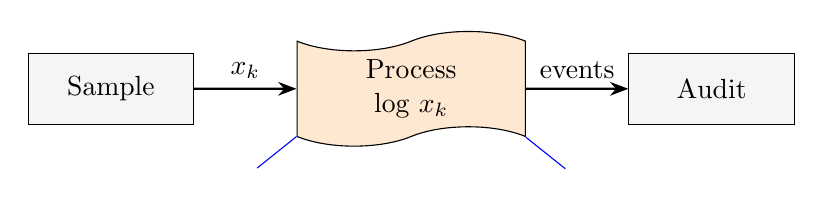
\begin{tikzpicture}[
  >=Stealth,
  node distance=13mm,
  block/.style={draw,minimum width=21mm,minimum height=9mm,fill=gray!8},
  log/.style={tape,draw,tape bend height=7pt,minimum width=29mm,
    minimum height=12mm,fill=orange!18,align=center},
  flow/.style={->,thick}
]
  \node[block] (sample) {Sample};
  \node[log,right=of sample] (trace) {Process\\log $x_k$};
  \node[block,right=of trace] (audit) {Audit};
  \draw[flow] (sample) -- node[above] {$x_k$} (trace);
  \draw[flow] (trace) -- node[above] {events} (audit);
  \draw[thin,blue] (trace.south west) -- ++(-5mm,-4mm);
  \draw[thin,blue] (trace.south east) -- ++(5mm,-4mm);
\end{tikzpicture}
\end{document}
